\documentclass[11pt]{amsbook}

\usepackage{../HBSuerDemir}	% ------------------------
\usepackage{wrapfig}
\usepackage{amsmath}


\begin{document}
% ++++++++++++++++++++++++++++++++++++++
\hPage{b1p2/481}
% ++++++++++++++++++++++++++++++++++++++

\begin{wrapfigure}{R}{0.45\textwidth}
	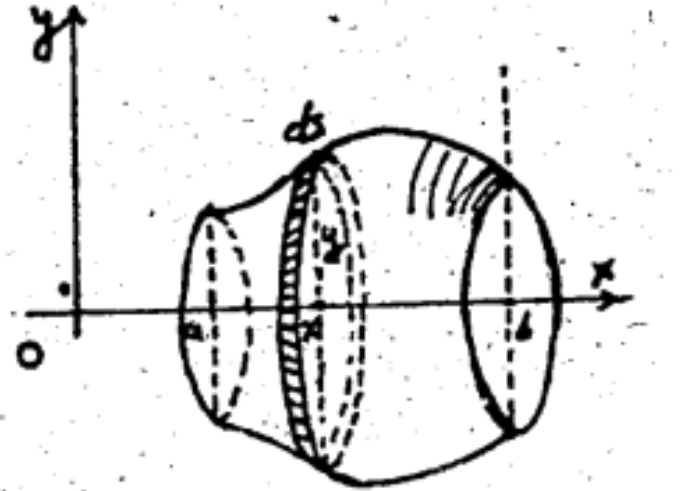
\includegraphics[width=0.40\textwidth]{images/b1p2-481}
	  \vspace{-20pt}
\end{wrapfigure}
\noindent cone whose lateral area is \vspace{10pt} \\
${ox} = 2\pi y , dS_{oy}=2\pi xds $ \vspace{10pt} \\ 
which by integration gives \vspace{10pt} \\
$S_{ox} = 2\pi \int_{a}^{b} \! y(x) \, \hDif s , S_{oy} = 2\pi \int_{c}^{d}\! x(y)$ \vspace{10pt} \\
If the curve is given by parametric equation we have 
$$ 
S_{ox} = 2\pi \int_{t_1}^{t_2} \! y\sqrt{x^2+y^2} \, \hDif t , 
S_{oy} = 2\pi \int_{t_1}^{t_2} \! x\sqrt{x^2+y^2}\, \hDif t 
$$
\begin{exmp}
Compute the surface area of the surface genarated when the curve 
\[y= \sqrt{x} , x\in (1,4)\]
is rotated abount x-axis.
\end{exmp}

\begin{hSolution}
  \begin{equation}
    \begin{split}
      S_{ox} &= 2\pi \int_a^b \! y \, \hDif s = 2\pi \int_1^4 \! y\sqrt{1+y^2} \, \hDif x \\
      &= 2\pi \int_1^4 \! \sqrt{x} \sqrt{1+\frac{1}{4x}} \, \hDif x = \pi \int_1^4 \! \sqrt{1+4x} \, \hDif x \\
      &= \hPairingParan{\frac{\pi}{6}} \hPairingParan{17\sqrt{17}-5\sqrt{5}}
    \end{split}
  \end{equation}
\end{hSolution}

\begin{exmp}{}
  Compute the area of the surface obtained when the curve 
  $$x = 3t\hPairingParan{t-2} , y = 8t^\frac{3}{2}$$
  is rotated abount x-axis.
\end{exmp}

\begin{hSolution}
  \begin{equation}
    \begin{split}
      S_{ox} &= 2\pi \int_0^1 \! y(t)\sqrt{x^2+y^2} \, \hDif t \\
      &= 2\pi \int_0^1 \! 8t\sqrt{t} \sqrt{(6t-6)^2 +12^2t} \, \hDif t \\
      &= 96\pi \int_0^1 \! t\sqrt{t} \hPairingParan{t+1} \, \hDif t = \frac{2304}{5} \pi
    \end{split} 
  \end{equation}
\end{hSolution}
% =======================================================
\end{document}  